\chapter{Proposed Solution}

\begin{chapquote}{Jim Barksdale}
If we have data, let’s look at data. If all we have are opinions, let’s go with mine.
\end{chapquote}

\section{Introduction}

Perform a data-driven analysis required to develop a collection of tools
to run in a lightning network node with daily activity. 
This section describes an open-source framework for defining and collecting
lightning network metrics.

Therefore, to implement this framework an analysis of the state 
of the art was required (described in Section \ref{sec:problem_and_state_of_the_art})
to better understand what information are more difficult 
to get from a researcher's point of view.

From our preliminary study, we found that information on how a node performs 
on a daily basis are difficult to get, due to the following problems:
\begin{itemize}
    \item Requires a direct interaction with \emph{node operators};\footnote{node operators are people that own a 
        lightning node that points to help the network in routing payments.}
    \item Data collection of this kind can leak private data, and node operators
        do not want to be exposed to this risk.
\end{itemize}

So, to work around these problems our proposal defines in a 
public manner what data will be collected, and how these will be analysed. This 
definition process is done through a lnmetrics Request for Comments (RFC) 
called \emph{lnmetrics RFC}. Then, after the data are defined, the collection 
of this data is done with a public server with public API with the possibility 
to self-hosting the server on hardware with at least a Raspberry PI 2 capability.

In addition, to incentives node operators to provide and share the 
information with one of the public servers available we write the tool that 
collect the information on the lightning node with the possibility to run 
in an offline mode, and only if and when the node operators want the data 
are shared with one of the servers chosen (or more than one server).
One of the reasons that make the possibility to run in an offline mode a good
the incentive for node operators to be part of the research is that they 
are seeking a tool to analyse the node performance to increase the profit of
their node.

The Figure \ref{fig:lnmetrics_process} shows as the general process of propose 
a solution with our framework looks like, where the steps are:

\begin{figure}
    \begin{center}
      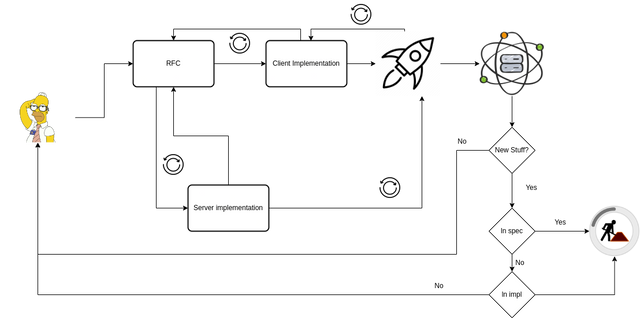
\includegraphics[scale=0.7]{imgs/lnmetrics-workflow-drawio.png}
    \end{center}
    \caption{Example of a process that uses lnmetrics.}
    \label{fig:lnmetrics_process}
\end{figure}

\begin{enumerate}
    \item {\bf Data Definition}: Should be the first step of the process in order
        to define clearly the scope of the data collection;
    \item {\bf Client Implementation}: After a first draft of the data model is defined,
        the next step should be the implementation of the tools that can collect 
        the data. This step could require going back to the previous step and change 
        part of the data model.
    \item {\bf Analysis Implementation}: Could be done in parallel with the Client implementation,
        and as in the client's case, the analysis of the data collected can bring to rethink the data model
        and return to step 1.
    \item {\bf RFC proposal}: When the data model and the code are in a stable phase,
        the metric can be proposed with an RFC and the discussion between the people interested
        can be done, but these steps can require to introduce changes in one or more of the previous steps;
    \item {\bf Possible Proposal}: After the RFC is discussed the data analysis can bring to some 
        official proposal to the lightning network protocol or to one of the lightning network implementations.
\end{enumerate}

In Section \ref{sec:demo} the process of our case study is discussed.

\section{LNMetrics Request for Comments (RFC)}

The LNMetrics Request for Comment (RFC) proposed is a more general idea of what 
it is already been done in the Lightning Network protocol definition. 
This RFC is pointing to having the data description of what data are collected 
and how these data are used. It is not trying to define a 
standard of metrics for the lightning network, 
but more to incentives discussion between people to achieve a better result.

\subsection{Data Definition}
\label{sec:data_definition}

Data definition is the most important part to propose a solution to a problem 
that required data analysis. Therefore, the data definition is a core 
part of the lnmetrics RFC process as the Figure \ref{fig:lnmetrics_process}
shows, and the process to propose a new \emph{metric} is composed of 
the following parts:

\begin{itemize}
    \item {\bf Metric Introduction}: An Introduction of the area that the metrics are targeting;
    \item {\bf Input Metric}: Data definition of the data that the researchers need. The data definition is done through a \emph{JSON schema}, and
    \item {\bf Output Metric}: Data definition of the data that the research point to return as a result. 
\end{itemize}

Ideally, the Metric proposal needs to be supported by a reference implementation to 
allow people to be part of the research by running the tool provided, and 
to support the RFC discussion.

However, at this time the problem on how to easily integrate new metrics inside the 
existing code is an open problem, and a possible solution is to allow the server 
described in Section \ref{sec:lnmetrics_server} to support a \emph{plugin protocol}
that allows any person to extend the existing server with additional features and leave to the user 
the decision on how to implement the client as described in the Section \ref{sec:lnmetrics_client}.
In conclusion, when the new metric has been proposed inside the RFC a discussion between interested 
group of people needs to be done to try to improve and verify the proposal, but if this is not possible
the proposal can be accepted directly by providing a reference implementation of the metrics proposed.

\section{Data Collection with LNMetrics Client}
\label{sec:lnmetrics_client}

An LNMetrics client is a generic concept of a tool that can collect one or more metrics 
defined inside the RFC, and allow a node operator or anyone that runs a lightning node
to collect data and share it with an analysis system described in Section \ref{sec:lnmetrics_server}.
To support our proposal a generic solution implemented in \emph{Go language} is provided 
and available on Github at \url{https://github.com/LNOpenMetrics/go-lnmetrics.reporter}, where we was able 
to provide a generic solution and allow the support of a generic metric concept 
by implementing the metric as an interface defined as the Code \ref{code:lnmetric_client_inter} shows.

\begin{lstlisting}[language=go, basicstyle=\small,
                  caption={Metric interface provided in our client reference implementation.}, 
                  label={code:lnmetric_client_inter}]
// All the metrics need to respect this interface
type Metric interface {
    // return the unique name that the metrics have
    MetricName() *string
    // called when the metrics are initialised from 
    // the lightning node
    OnInit(lightning client.Client) error
    // called when the node is shutting down
    OnStop(msg *Msg, lightning client.Client) error
    // used to make the actual status of the metrics
    // persistent
    MakePersistent() error
    // called when the metrics are ready to be published
    UploadOnRepo(client *graphql.Client, 
        lightning client.Client) error
    // called when the metrics for the specific node 
    //needs to be initialised on the server
    InitOnRepo(client *graphql.Client, 
        lightning client.Client) error
    // call that the lightning node used when it is 
    // time to update the metrics with new data
    Update(lightning client.Client) error
    // a more specific method to be able to call the 
    // update metrics with a specific message that allows 
    // to pass more information to the update method
    UpdateWithMsg(message *Msg, 
        lightning client.Client) error
    ToMap() (map[string]any, error)
    ToJSON() (string, error)
    // allow to perform data migration from an old 
    // data version to a new one
    Migrate(payload map[string]any) error
}
\end{lstlisting}

The LNMetrics client provided uses the core lightning plugin API
that allows us to easily integrate the client with the core lightning daemon 
and run the metrics client as part of the node itself. 
In addition, to allow an easy development of the plugin a 
Go API for core lightning is also provided, and available on 
Github at \url{https://github.com/vincenzopalazzo/cln4go}.

When the plugin is started a setup operation is performed, by creating a 
metrics database where the plugin makes persistent the information 
across node restarts, and also to support the offline mode feature. 
The chosen database is \emph{leveldb} that is a \emph{NO SQL} database 
that allow to store an efficient way data as key-value and preserve
the disk space with a compression algorithm built into the database itself.
Our client implementation is heavily based on the 
compression feature to preserve and allow anyone to 
run the tool. 
In Figure \ref{fig:lnmetrics_diskspace} it is shows how much space is 
consumed by the database in our two test machines. 

\begin{figure}
    \begin{center}
    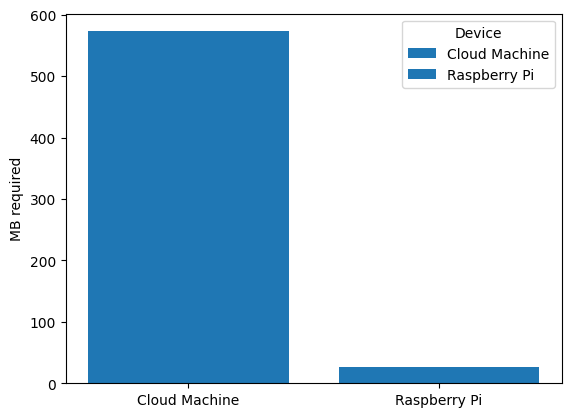
\includegraphics[scale=0.7]{imgs/disk_space_servers.png}
    \end{center}
    \caption{LNMetrics database size by instances.}
    \label{fig:lnmetrics_diskspace}
\end{figure}

\begin{itemize}
    \item {\bf Cloud machine}: Disk space consumed by the lnmetrics 
        system on the cloud machine to store more than 1 year of metrics data;
    \item {\bf Raspberry PI 3}: Disk space consumed by the lnmetrics system
        on a Raspberry PI to store 4 months of metrics data.
\end{itemize}

In Section \ref{sec:demo} more information about the data collected is discussed.

\section{LNMetrics Data Analysis}
\label{sec:lnmetrics_server}

After the data are collected by the LNMetrics client described in \ref{sec:lnmetrics_client}
we propose to aggregate the data in a server with public API where the data are 
publicly accessible to everyone. In this section, there is a discussion of 
the server solution provided.

\subsection{Design Choice}

The choice to aggregate the data collected in a peer-to-peer system in a public 
server may sound a little bit odd, but the lnmetrics framework is designed in a 
way to keep every concept separate as the Figure \ref{fig:lnmetrics_architecture} 
shows. The analysis system is independent of the client that collects and reports
the data and the only information shared across the systems is the data format, 
that in our design is done through the lnmetrics RFC.

\begin{figure}
    \begin{center}
    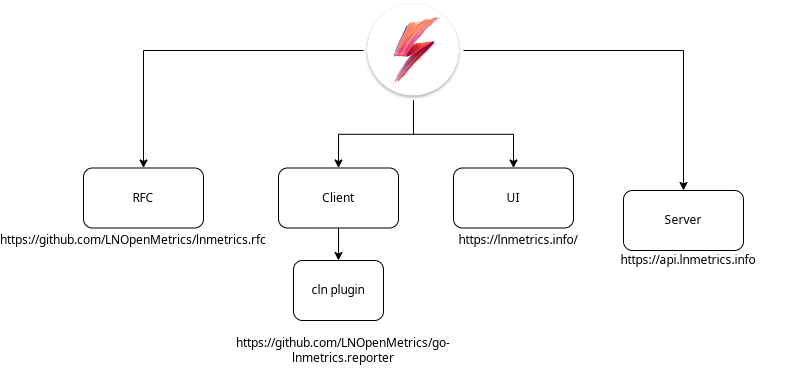
\includegraphics[scale=0.5]{imgs/lnmetrics-architecture.drawio.png}
    \end{center}
    \caption{LNMetrics architecture design diagram.}
    \label{fig:lnmetrics_architecture}
\end{figure}

Our choice to provide the lnmetrics server as a method to analyse the data is to 
give one tool to organisations and Universities to collect the data in a centralised
way to simplify the analysis step. However, our client implementation is able
to compute the metric analysis in a local environment, and allow the owner
of the node to inspect the result calculated without sharing the data with the centralised
server.

\subsection{API Description}

The server API uses the \emph{GraphQL protocol} that allows a flexible way to fetch
a subpart of the data from the server. In particular, the GraphQL Protocol uses
a concept of \emph{Query} where it is possible to specify only the data that the 
caller wants to know and avoid receiving all the JSON as a response. The motivation of this 
choice is to improve the efficiency of the server and speed up the performance when the caller needs 
access to a subset of information and not to the full raw content. 

However, the downside of this approach is that with the GraphQL protocol the learning 
curve for a user is more height that a normal Rest protocol, for this reason for our
case study a python library that implements a wrap of the server API is provided 
and available on Github at \url{https://github.com/LNOpenMetrics/py-lnmetrics.api}. 

In conclusion, we provided a public API available at \url{https://api.lnmetrics.info} with 
a web site available at \url{https://lnmetrics.info} that provide access to the 
lnmetrics RFC, and some analysis of the case study described in the 
following sections.

\section{Local Reputation Metric}
\label{sec:demo}

This section is described our case study that uses the lnmetrics framework to 
define a local reputation of the node to provide a solution to a problem 
that we had while we were building our lightning node on the Bitcoin network.

The local reputation described in this section is trying to have anought data 
to support a lightning network user during the initial phase, and 
helps to define some criteria to discover a \emph{good lightning node} 
where it is possible to initialise a channel. In addition, with these local reputations 
system it is possible help node management tools like \emph{clboss}\cite{clboss}
to score the channel, and have some additional information at runtime.

\subsection{Data Definition}
\label{sec:data_definition_datadef}

The first step that we have done is to start to design our data model by analysing
the data that we were able to get from the core lightning node. Our first version
of the data model is available on Github at \cite{lnmetrics_localreputation}. 
Moreover, the data are split into two main part divided as follow:

\begin{enumerate}
    \item {\bf Lightning Node performance information}: The performance of the node that it is running
        the metrics, including
        \begin{itemize}
           \item Operative System information;
           \item The number of channels that the node has;
           \item The number of forwards payments that the node has performed in the 
               last 30 minutes;
           \item The current lightning fee that the node has to 
               forward a payment.
        \end{itemize}
    \item {\bf Performance for each channel}:
    \begin{itemize}
        \item If the node is online at the moment of the check;
        \item The current lightning fee of the channel to forward a payment through it;
        \item The number of payments that are forwarded in the last 30 minutes through this specific 
            channel;
        \item The channel direction, where for each lightning channel there will be two items: one of 
            inbound connection, and another one for outbound connection. In this way it is possible to 
            try to estimate the usable direction of the channel.
    \end{itemize}
\end{enumerate}

When the client provides the data to the analysis system the following metric output is calculated:

\begin{itemize}
    \item Lightning node up time scoring divided by period is calculated;
    \item Lightning channel forwards payment scoring divided in \emph{success}, \emph{failure} and \emph{local failure}
        is calculated, where the local failure is how many forwards are failing caused to some lightning node problem,
        e.g the node that is running the metrics has no channel with enough outbound capacity. 
    \item For each channel the previous information is calculated for this particular channel.
\end{itemize}

A more detailed description of the metric output is provided on Github as RFC with the JSON schema 
of the data just described, and we avoid reporting the full code example due to the size of the 
JSON schema. 

\subsection{Reference Implementation}

The client implementation of the local reputation described in \ref{sec:data_definition_datadef} 
is provided inside our Go Lang reference implementation discussed in \ref{sec:lnmetrics_client},
and this section includes a practical description of how to use it.
Therefore, the client implementation is a plugin for core lightning able to 
run as part of the daemon itself, so to run the plugin the core lightning
need to know the path of the plugin binary, and an example of the command is shown in
the code \ref{code:cln_with_lnmetrics}.

\begin{lstlisting}[language=bash, basicstyle=\small,
                  caption={Command to run the core lightning daemon with the lnmetrics plugin enabled.}, 
                  label={code:cln_with_lnmetrics}]
>> lightningd --plugin=/<path to the plugin binary>/go-lnmetrics
\end{lstlisting}

When core lightning will finish to set up the environment, a directory inside 
the core lightning directory with the name \emph{metrics} is created, and 
it is the home of the lnmetrics plugin where all information is stored. 
In addition, a metrics.log file is created to be able to debug the 
plugin without interacting with the core lightning log daemon.

After the node is running the plugin will perform the initialisation 
of the information required by the local reputation described before, and 
then every 30 minutes the plugin will perform the update of the metrics by 
get the last information by querying the core lightning node. 

However, if the plugin is run with the command \ref{code:cln_with_lnmetrics}
the plugin will run in offline mode, and this means that the metrics are kept 
only in the local machine where the node is running, and not shared with the server. 
Therefore, to share the data with the server the API URL need to be specified,
as the Code \ref{code:cln_with_lnmetrics_url} shows.

\begin{lstlisting}[language=bash, basicstyle=\small,
                  caption={Command to run core lightning with the lnmetrics plugin an publish the data.}, 
                  label={code:cln_with_lnmetrics_url}]
>> lightningd --plugin=/<path to the plugin binary>/go-lnmetrics \ 
--lnmetrics-urls=https://api.lnmetrics.info/query
\end{lstlisting}

More endpoints can be specified by appending them to the lnmetrics-urls command line operation separate by a comma.

In conclusion, it is possible to query the plugin by interacting with the core lightning command line interface,
and call the following method provided by the plugin:

\begin{itemize}
    \item {\bf raw-local-reputation}: Query the last input data collected by the plugin in the last 30 minutes; 
        the data format of this plugin is described inside the \cite{lnmetrics_localreputation};
    \item {\bf local-reputation}: Query the last local reputation calculate on the data provided by the 
        raw-local-reputation command and the data format is described in \cite{lnmetrics_localreputation}.
\end{itemize}

\subsection{Data Analysis}

When the client is running with an endpoint as in the Code \ref{code:cln_with_lnmetrics_url},
the metrics are collected and reported to the server provided. The server instance exposes an
endpoint that accepts a \emph{Mutation}\footnote{A Mutation query in the GraphQL is a special query that points to mutate the state of the server.} query,
as the Code \ref{code:lnmetrics_mutation} shows.

\begin{lstlisting}[language=graphql, basicstyle=\small,
                  caption={Mutation query call by the client to initialise the metric on the server.}, 
                  label={code:lnmetrics_mutation}]
mutation {
    initMetricOne(node_id: "...", payload: "{....}", signature: "...") {
        node_id
        ...
    }
}
\end{lstlisting}

Where the input parameters of the mutation are:

\begin{itemize}
    \item {\bf node\_id}: The node public key used as node identifier on the lightning network;
    \item {\bf payload}: The JSON payload of the metric that the node is publishing;
    \item {\bf signature}: The signature of the JSON payload sent as input to be able to verify that the 
        payload is sent by the node with the public key provided.
\end{itemize}

The algorithm to sign the payload is a custom algorithm provided by the major
lightning implementation, and we provide our Go implementation available 
at \url{https://github.com/LNOpenMetrics/lnmetrics.utils}.

When the metrics is accepted and verified by the server, it will perform the analysis of the 
metric provided and calculate the metrics output described in \ref{sec:data_definition_datadef}, 
and then the metrics are available through the server endpoint. In addition, our python client 
provides an easy API to access any server instances. The Code \ref{code:lnmetrics_python_api}
provide a runnable example.


\begin{lstlisting}[language=python, basicstyle=\small,
                  caption={Python script to show a runnable example of our Python wrapper API usage.}, 
                  label={code:lnmetrics_python_api}]
from lnmetrics_api import LNMetricsClient

client = LNMetricsClient(service_url="https://api.lnmetrics.info/query")
nodes = client.get_nodes(network="bitcoin")
print(f"The nodes on the server are {nodes}")
metric = client.get_local_score_output(network="bitcoin", 
               node_id="03e2408a49f07...")
print(f"The local score of the node is {metric}")
\end{lstlisting}

In addition, we use the python API to write a Jupyter Notebook available at \url{https://github.com/LNOpenMetrics/local-reputation-analysis}
where we make an initial analysis of the data collected, and we discuss 
the result in the remaining section.

\subsubsection{Nodes Up time}
\label{sec:node_uptime}

In this section is discussed the result of the analysis of metrics provide by 
the node available on the cloud server.

\begin{figure}
    \begin{center}
      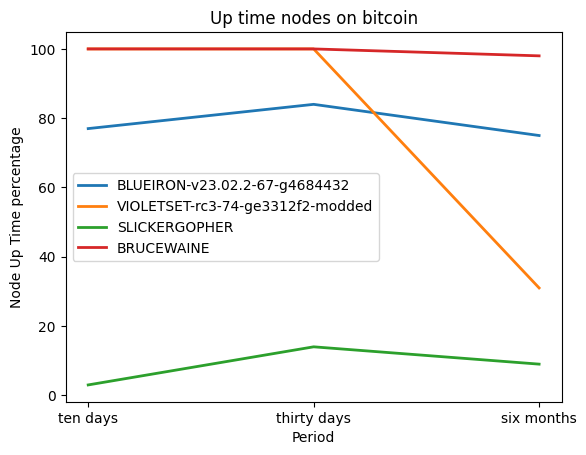
\includegraphics[scale=0.7]{imgs/bitcoin_uptime.png}
    \end{center}
    \caption{Lightning Node up-time scoring on the Bitcoin Network calculate by the cloud machine.}
    \label{fig:lnmetrics_uptime_bitcoin}
\end{figure}

\begin{figure}
    \begin{center}
      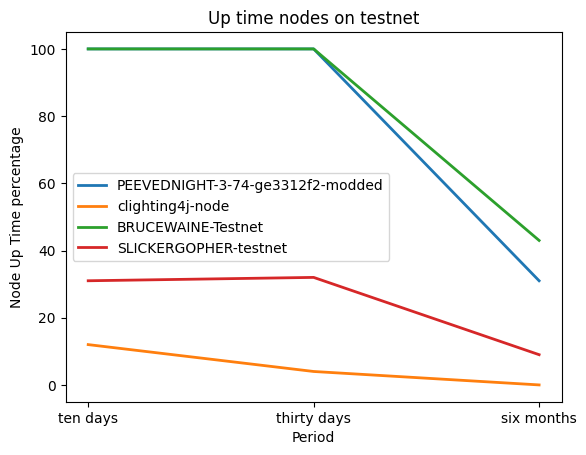
\includegraphics[scale=0.7]{imgs/testnet_uptime.png}
    \end{center}
    \caption{Lightning Node up-time scoring on the Testnet Network calculate by the cloud machine.}
    \label{fig:lnmetrics_uptime_testnet}
\end{figure}

Figure \ref{fig:lnmetrics_uptime_bitcoin} shows the up-time scoring of the nodes that 
are sharing data on the server every 30 minutes, so the node with the 100\% up-time 
is the node that is always online. Therefore, from this analysis, we can 
see some kinds of patterns where there are nodes that are not always online such as the one 
with the alias \emph{SLICKERGOPHER}. In fact, 
this node is not a routing node, but it is just a node that is run by a casual user.

In conclusion, in the Figure \ref{fig:lnmetrics_uptime_testnet} is
shows the up-time of the nodes in the Testnet network, where we can see also 
this difference between nodes is always online and casual users.

\subsubsection{Forwards Rating}
\label{sec:forwards_rating}

In Section \ref{sec:node_uptime} is analysed the up-time of the nodes and we 
noted that it is possible note at least two kinds of nodes that are: 

\begin{itemize}
    \item {\bf Routing Node}: Nodes that are always online;
    \item {\bf Casual User} Node Node Node that are not always online.
\end{itemize}

Therefore, just by analysing the up-time of the node it is possible to extract useful information 
in order to drive some decisions at runtime. However, know just the 
up-time of a node is not enough to estimate if a node is a good node for the public network 
because a routing node that is always online needs to have some activity and this activity 
should not be dangerous for the network.
For this reason, in this section, we use the forwards rating to measure the activity of a node 
by analysing how many payments are forwarded by the routing node under analysis and for our analysis 
we take into consideration two nodes, one in the Bitcoin Network and the other one in the Testnet network.

\begin{itemize}
    % FIXME: there is a better way to go to the next line, but I am not able to find this better way!
    \item {\bf BLUEIRON}: The lightning node with the public key 024b9a1fa8e006f1e3937f6-\\5f66c408e6da8e1ca728ea43222a7381df1cc449605 for the Bitcoin Network;
    \item {\bf BRUCEWAINE-Testnet}: The lightning node with public key 030b686a163aa2bba0-\\3cebb8bab7778fac251536498141df0a436d688352d426f6 for the Testnet Network.
\end{itemize}

In Figure \ref{fig:bitcoin_vs_testnet_forwards} there is an analysis of the forwarded payments by 
the node under analysis for each network, and in Figure \ref{fig:bitcoin_vs_testnet_channels_size} there is an 
analysis of the size of the node during the period that includes the number of channels that the node 
has.

Therefore, from this comparison, we can see that the activity on the Bitcoin network 
is the order of magnitude bigger that the activity on the Testnet network, also if the 
side of the node is close to be the same. This shows that the activity on the Bitcoin network and 
the activity on the Testnet network are very different, and this may impact the proposal evaluation 
that is dependent on the network such as the local scoring proposed by the solution to solve 
the Jamming Attack discussed on the Section \ref{sec:jamming}.

\begin{figure}[H]
    \begin{center}
        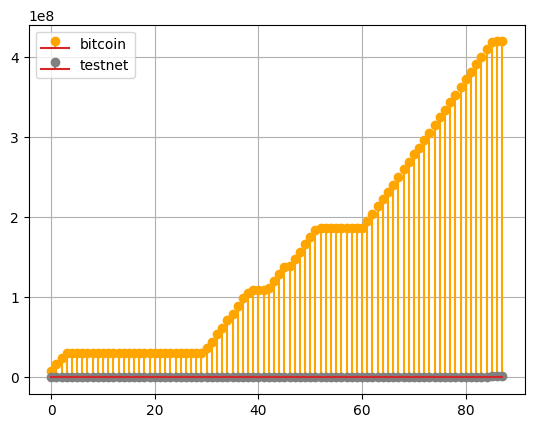
\includegraphics[scale=0.7]{imgs/bitcoin_vs_testnet_forwards.png}
    \end{center}
    \caption{Comparison between networks of the Lightning Node forwards scoring.}
    \label{fig:bitcoin_vs_testnet_forwards}
\end{figure}

\begin{figure}[H]
    \begin{center}
      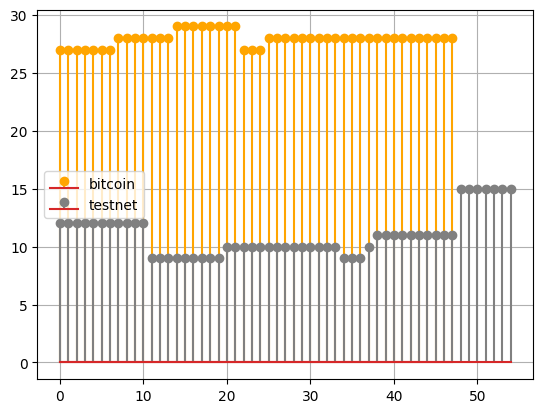
\includegraphics[scale=0.7]{imgs/bitcoin_vs_testnet_channels_size.png}
    \end{center}
    \caption{Comparison between networks of the Lightning Node size.}
    \label{fig:bitcoin_vs_testnet_channels_size}
\end{figure}

However, with Figure \ref{fig:bitcoin_forwards_rating} we can see how also the success forwards scoring 
on the Bitcoin network is close to the 5\% of the total forwards performed in the last 6 months. One of the main 
reasons for this result can be the probing techniques that some nodes are using in order to estimate the exact capacity
of the channel before performing the path-finding algorithm. In these probing techniques, the node that wants to make payments
will send fake payments that are already failed with an increasing amount just to know if the channel where this 
payment is directed is able to forward it. The lightning node that is receiving this forward payment is not able to 
note that it is a fake payment due to the onion routing discussed in Section \ref{sec:onion_routing}.
So, just looking at the global forwards scoring 
of a node, it is not enough because the failure scoring will be always a big part of this analysis due to 
these probing techniques, but this information is useful to be able to filter nodes that forwards only payments 
that will fails payments, and are not local failure.


\begin{figure}
    \begin{center}
      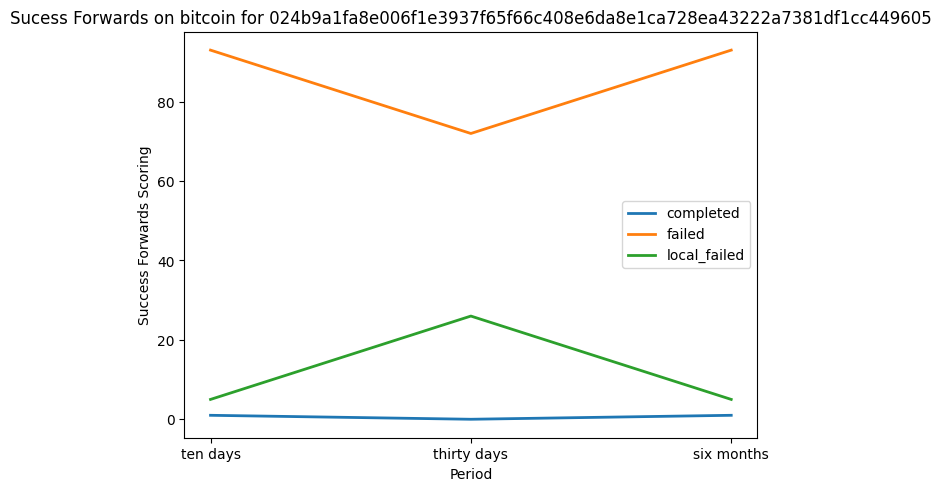
\includegraphics[scale=0.7]{imgs/bitcoin_forwards_rating.png}
    \end{center}
    \caption{Forwards Scoring for the Lightning network node on the Bitcoin Network.}
    \label{fig:bitcoin_forwards_rating}
\end{figure}

% FIXME: we could add a small analysis of the forwards scoring for each channels


